\documentclass[../piano-di-progetto.tex]{subfiles}

\begin{document}

  \subsection{Verifica e collaudo}

  \subsubsection{Prospetto orario}
  Nel periodo di Verifica e collaudo, la distribuzione oraria è la seguente:
  \begin{table}[H]
    \centering
    \begin{tabular}{lccccccc}
      Sofia Bonomi              & 2           & 5           & -          & -           & 7           & 10          & 24           \\
      Enrico Buratto            & -           & 5           & -          & 2           & 9           & 7           & 23           \\
      Ian Nicolas Di Menna      & 4           & -           & -          & -           & 7           & 10          & 21           \\
      Alessandro Franchin       & 4           & -           & -          & -           & 9           & 10          & 23           \\
      Enrico Galdeman           & -           & -           & -          & 6           & 9           & 10          & 25           \\
      Nicholas Miazzo           & -           & 5           & -          & -           & 7           & 10          & 22           \\
      Marco Nardelotto          & -           & 5           & -          & 4           & 7           & 9           & 25           \\
      \textbf{Ore totali ruolo} & \textbf{10} & \textbf{20} & \textbf{0} & \textbf{12} & \textbf{55} & \textbf{66} & \textbf{163} 
    \end{tabular}
    \caption{Distribuzione oraria del periodo di Verifica e collaudo}
  \end{table}


  Per facilitare la lettura della distribuzione oraria, i dati vengono rappresentati graficamente il seguente istogramma:
  \begin{figure}[H]
    \centering
    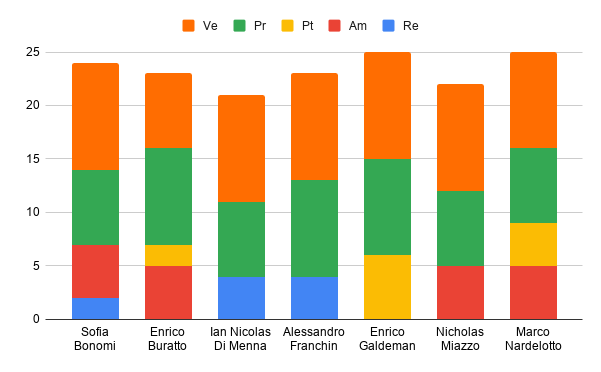
\includegraphics[width=12cm]{img/ore-verifica.png}
    \caption{Istogramma della distribuzione oraria del periodo di Verifica e collaudo}
    \label{fig:ore-componente-verifica}
  \end{figure}

  \subsubsection{Prospetto economico}
  In questo del periodo, la suddivisione oraria e i costi per ruolo è la seguente:

  \begin{table}[H]
    \centering
    \begin{tabular}{lcc}
      Ruolo           & Ore previste & Costo               \\
      Responsabile    & 10           & € 300,00            \\
      Amministratore  & 20           & € 400,00            \\
      Analista        & -            & € 0,00              \\
      Progettista     & 12           & € 264,00            \\
      Programmatore   & 55           & € 825,00            \\
      Verificatore    & 66           & € 990,00            \\
      \textbf{Totale} & \textbf{163} & \textbf{€ 2.779,00}
    \end{tabular}
    \caption{Prospetto economico del periodo di Verifica e collaudo}
  \end{table}


  Per facilitare la lettura della suddivisione oraria per ruolo, i dati vengono rappresentati graficamente mediante il seguente areogramma:
  \begin{figure}[H]
    \centering
    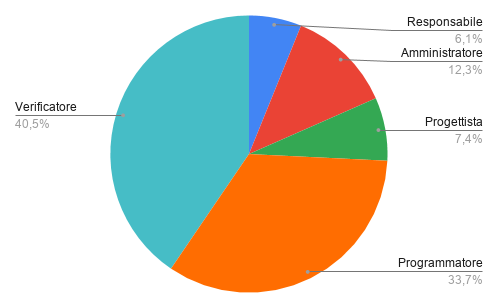
\includegraphics[width=12cm]{img/ruoli-verifica.png}
    \caption{Areogramma della suddivisione dei ruoli del periodo di Verifica e collaudo}
    \label{fig:ore-ruolo-verifica}
  \end{figure}

\end{document}
